\documentclass[11pt]{article}
\usepackage{cse216,hyperref}
% use the tikz package to draw automata
\usepackage{tikz}
\usetikzlibrary{arrows,positioning,automata}
\def\title{HW 6}
\begin{document}
\maketitle

\section*{Due November 10 at 3:00 pm}

\textbf{(2 questions, 55 points total)}

\begin{qunlist}

  \q{30}{LTL and CTL}\\
  Consider the following Kripke structure $M$ with atomic propositions $p$ and $q$:

  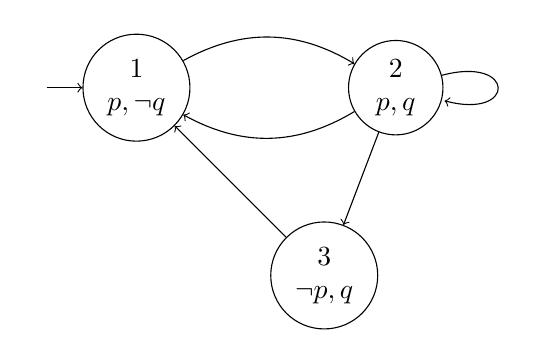
\begin{tikzpicture}[node distance=2cm]
    \node[state, initial, initial text=, align=center] (s0) {1\\$p, \lnot q$};
    \node[state, right= of s0, align=center] (s1) {2\\$p , q$};
    \node[state, below right= of s0, align=center] (s2) {3\\$\lnot p , q$};

    \path[->]
    (s0) edge[bend left] (s1)
    (s1) edge[bend left] (s0)
    (s1) edge[loop right] (s1)
    (s1) edge (s2)
    (s2) edge (s0);
  \end{tikzpicture}

  \begin{qparts}
  \item
    Does $M \models GFq$? Why or why not?

    \begin{answer}
      yes. all states can always eventually end up in a state that has \(q\).

    \end{answer}

  \item
    Does $M \models G(\lnot q \; U \, p)$? Why or why not?

    \begin{answer}
      state 3 has \(q\) and \(\neg p\), which means at this state the condition \(\neg q ~ U ~ p\) is false
    \end{answer}

  \item
    Does $M \models G(q \rightarrow XX p)$? Why or why not?

    \begin{answer}
      no because from state 2 there exists a path where 2 steps from state 2 has \(\neg p\). the path is 2 2 3.

    \end{answer}

  \item
    Does $M \models EG p$? Why or why not?

    \begin{answer}
      yes because there always exists a path from any node that has \(p\) hold globally, the one that loops forever on state 2.

    \end{answer}

  \item
    From which states does the formula $EX q$ hold?

    \begin{answer}
      only 3 does not satisfy this since there is no immediate next state to which it can transition where \(q\) holds.
    \end{answer}

  \item
    Does $M \models AF (EX q)$? Why or why not?

    \begin{answer}
      yes. all states always finally have a state where their next state makes \(q\) true.
    \end{answer}
  \end{qparts}


  \q{25}{B\"uchi Automata}\\
  Consider the following B\"uchi automaton $B$:

  \begin{tikzpicture}[node distance=2cm]
    \node[state, initial, initial text=, align=center] (s0) {};
    \node[state, above right= of s0, align=center] (s1) {};
    \node[state, right= of s1, align=center, accepting] (s2) {};
    \node[state, below right= of s0, align=center, accepting] (s3) {};

    \path[->]
    (s0) edge node[above left] {$p$} (s1)
    (s1) edge[bend left] node[above] {$p$} (s2)
    (s1) edge[loop above] node[above] {$\lnot p$} (s1)
    (s2) edge[bend left] node[below] {$\lnot p$} (s1)
    (s2) edge[loop above] node[above] {$p$} (s2)
    (s0) edge node[below left] {$p$} (s3)
    (s3) edge[loop below] node[below] {$\lnot p$} (s3);
  \end{tikzpicture}

  \begin{qparts}
  \item
    Does $B$ accept the trace $(p, \lnot p, p, \lnot p, \dots)$?

    \begin{answer}
      yes because the automata would visit the top accept state infinitely many times in this alternating trace.
    \end{answer}

  \item
    Does $B$ accept the trace $(\lnot p, \lnot p, \lnot p, \dots)$?

    \begin{answer}
      no because it would instantly reject. there isnt even an infinite trace starting with \(\neg p\)
    \end{answer}

  \item
    Does $B$ accept the trace $(p, \lnot p, \lnot p, \lnot p, \dots)$?

    \begin{answer}
      yes since the bottom branch would stay on the accepting node forever.

    \end{answer}

  \item
    Write an LTL formula satisfied by exactly the words accepted by $B$.

    \begin{answer}
      the bottom path is modeled by $$p \land \text{X}(\text{G } \lnot p)$$ and the top is modeled by $$p \land \text{G F } p$$ so the total automata is

      $$p \land (\text{X}(\text{G } \lnot p) \lor \text{G F } p)$$


    \end{answer}
  \end{qparts}

\end{qunlist}
\end{document}
